\input templates/header
\title[DS - Epidemic Dissemination]{\textbf{Distributed Algorithms}\\Epidemic Dissemination}

\begin{document}

\newcommand{\Value}{\mathit{value}}
\newcommand{\Time}{\fontvar{time}}
\newcommand{\Now}{\fontproc{now}}
\newcommand{\Random}{\fontproc{random}}
\newcommand{\Update}{\textsc{update}\xspace}
\newcommand{\Push}{\textsc{push}\xspace}
\newcommand{\Pull}{\textsc{pull}\xspace}
\newcommand{\ReplyPull}{\textsc{reply}\xspace}
\newcommand{\PushPull}{\textsc{pushpull}\xspace}
\newcommand{\ReplyPushPull}{\textsc{reply}\xspace}


\FrameTitle
\FrameContent

\section{Introduction}

\subsection{Motivation}

\begin{frame}{Data dissemination}

\structure{Problem}

\BIL
\item Application-level broadcast/multicast is an important building block
to create modern distributed applications

\BI
\item Video streaming
\item RSS feeds
\EI

\item Want efficiency, robustness, speed when scaling
\BI
\item \alert{Flooding} (reliable broadcast) is robust, but inefficient ($O(n^2)$)
\item \alert{Tree} distribution is efficient ($O(n)$), but fragile
\item \alert{Gossip} is both efficient $(O(n \log n))$ and robust, but has relative
  high latency
\EI

\item Scalability:
\BI
\item Total number of messages sent by all nodes
\item Number of messages sent by each of the nodes
\EI

\EIL

\note{

\BIL
\item What if you want to deliver a message to millions of nodes? 

\item You have to trade robustness (the ability to withstand a large number of 
failures) versus scalability (the ability of delivering messages to millions
of nodes).

\item Evaluating scalability cannot be focused just on the total number of
messages; even sending millions of messages from a single node is difficult.

\EIL

}

\end{frame}

\begin{frame}{Trade-offs}
	
\begin{figure}
	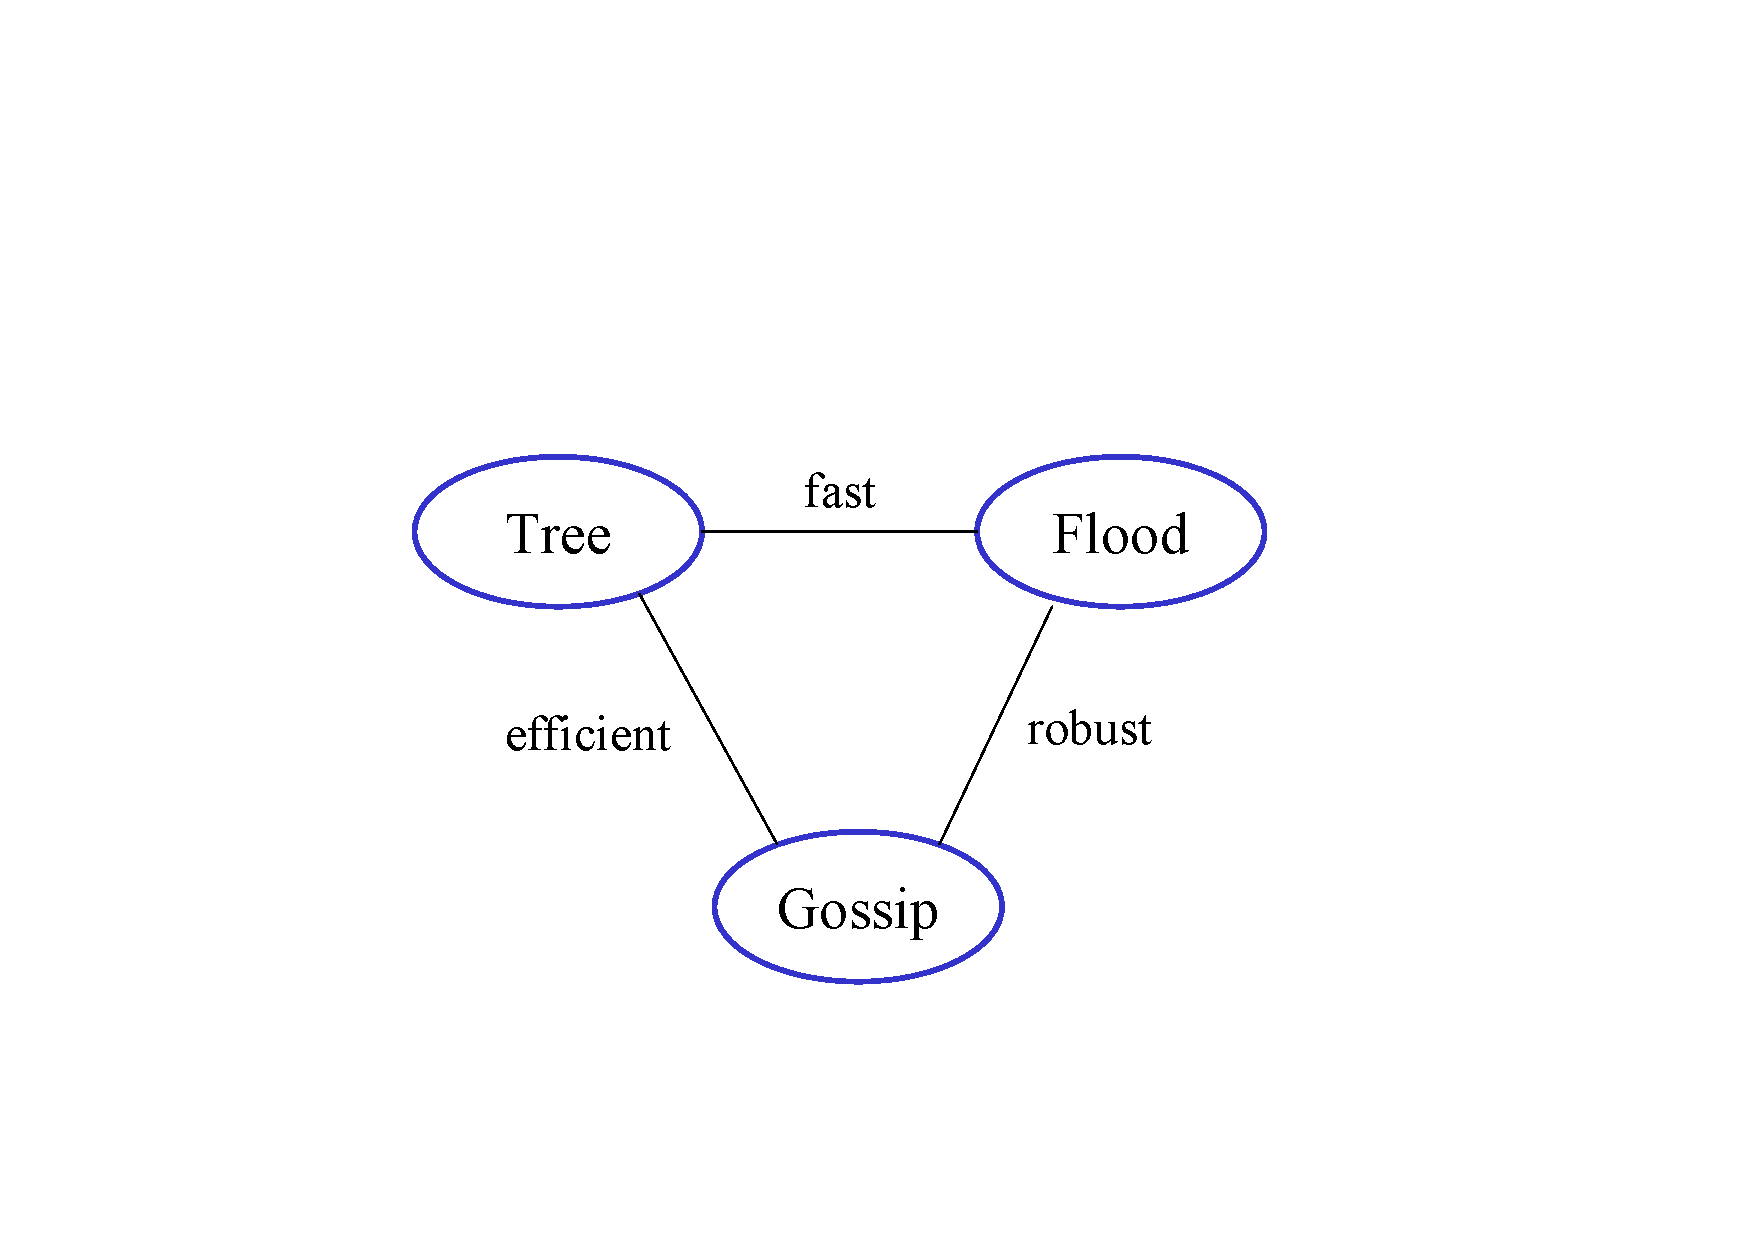
\includegraphics[width=10cm]{figs/05/tradeoffs}
	\caption{Courtesy: Robbert van Renesse}
\end{figure}
\end{frame}


\begin{frame}{Introduction}
	
\structure{Solution}

\BIL
\item Reverting to a probabilistic approach based on \alert{epidemics} / \alert{gossip}	
\item Nodes \alert{infect} each other trough messages
\item Total number of messages is less than $O(n^2)$
\item No node is overloaded
\EIL

But:

\BIL
\item No deterministic guarantee on reliability
\item Only probabilistic ones
\EIL

\end{frame}

\begin{frame}{History of the Epidemic/Gossip Paradigm}
	
\BIL
\item First defined by Alan Demers et al. (1987)
\item Protocols based on epidemics predate Demers' paper (e.g. NNTP)
\item '90s: gossip applied to the information dissemination problem
\item '00s: gossip beyond dissemination
\item 2006: Workshop on the future of gossip (Leiden, the Netherlands)
\EIL	
	
\begin{figure}

\includegraphics[width=0.20\textwidth]{figs/05/demers}	
\qquad

\includegraphics[width=0.20\textwidth]{figs/05/poster}	
\end{figure}
	
\end{frame}

\begin{frame}{Reality check (1987)}
\structure{XEROX Clearinghouse Servers}
\BIL
\item Database replicated at thousands of nodes 
\item Heterogeneous, unreliable network
\item Independent updates to single elements of the DB are injected at multiple nodes
\item Updates must propagate to all nodes or be supplanted by later updates of the same element
\item Replicas become consistent after no more new updates
\item Assuming a reasonable update rate, most information at any given replica is “current”	
\EIL

\end{frame}

\begin{frame}{Reality check (today)}

\BIL
\item Amazon uses a gossip protocol to quickly spread information throughout the S3 system
\item Amazon's Dynamo uses a gossip-based failure detection service
\item The basic information exchange in BitTorrent is based on gossip
\EIL	

\end{frame}
	
\subsection{System model}

\begin{frame}{Basic assumptions}
	
\BIL

\item \alert{System is asynchronous}
	\BI
	\item No bounds on messages and process execution delays
	\EI
	
\item \alert{Processes fail by crashing}
	\BI
	\item stop executing actions after the crash
	\item We do not consider Byzantine failures
	\EI
	
\item \alert{Communication is subject to benign failures}
 \BI
 \item Message omission
 \item No message corruption, creation, duplication
 \EI
	
\EIL

\end{frame}

\begin{frame}{Data model}

\BIL	
\item We consider a database that is replicated at a set of $n$ nodes $\Pi =
\{ p_1, \ldots, p_n \}$
\item The copy of the database at node $p_i$ can be represented by a
time-varying partial function:
\[
  \Value_i: K \rightarrow V \cdot T
\]
where:
\BI
\item $K$ is the set of \alert{keys}
\item $V$ is the set of \alert{values}
\item $T$ is the set of \alert{timestamps}
\EI
\item The update operation is formalized as: $\Value_i(k) \gets (v, \Now())$
where \Now() returns a globally unique timestamp 
\EIL

\end{frame}

\subsection{Specifications}

\begin{frame}{Database Specification}
The goal of the update distribution process is to drive the system towards consistency:

\bigskip
\begin{definition}[Eventual consistency]
If no new updates are injected after some time $t$, eventually all correct nodes will
obtain the same copy of the database:
\[
 \forall p_i, p_j \in \Pi, \forall k \in K : \Value_i(k) = \Value_j(k)
\]
\end{definition}

\end{frame}

	
\begin{frame}{Probabilistic Broadcast Specification}

\structure{An alternative view}
	
\bigskip
\begin{block}{PB1 – \alert{Probabilistic validity}}
There is a given probability such that for any two correct nodes $p$ and
$q$, every message PB-broadcast by $p$ is eventually PB-delivered by $q$
\end{block}

\bigskip
\begin{block}{PB2 - \alert{Integrity}}
Every message is PB-delivered by a node at most once, and only if it was previously PB-broadcast
\end{block}

\end{frame}

\begin{frame}{Best-Effort Broadcast vs Probabilistic Broadcast}

\structure{Similarities}:

\BI
\item No agreement property
\EI

\structure{Differences}:

\BI
\item Probability in BEB is “hidden” in process life-cycle
\item Probability in PB is explicit	
\EI
	
\end{frame}	

\begin{frame}{Some simplifying assumptions}

\BIL
\item Every node knows $\Pi$ (the communication network is a full graph)
\item Communication costs between nodes are homogeneous
\item We assume there is a single entry in the database
 \BI
  \item We simplify notation ($\Value_i(k) \rightarrow \Value_i$)
  \item Managing multiple keys is more complex than adding \\
   $\textbf{foreach}\ k \in K$
 \EI
\EIL

\bigskip
\structure{To be relaxed later...}

\end{frame}

	
\subsection{Models of epidemics}
	
\begin{frame}{Models of epidemics}
	
\begin{definition}[Epidemiology]
\alert{Epidemiology} studies the spread of a disease or infection in terms of populations 
of infected/uninfected individuals and their rates of change
\end{definition}

\bigskip
\structure{Why?}
\BI
\item To understand if an epidemic will turn into a pandemic
\item To adopt countermeasures to reduce the rate of infection
 \BI
 \item Inoculation
 \item Isolation
 \EI
\EI

\end{frame}

\begin{frame}{SIR Model}

\begin{definition}[SIR Model -- Kermack and McKendrick, 1927]
An individual $p$ can be:
\BIL
\item \alert{Susceptible}: if $p$ is not yet infected by the disease
\item \alert{Infective}: if $p$ is infected and capable to spread the disease
\item \alert{Removed}: if $p$ has been infected and has recovered from the disease
\EIL
\end{definition}

\begin{figure}
	
\includegraphics[width=0.8\textwidth]{figs/05/model-sir}
\end{figure}

\end{frame}

\begin{frame}{SIR Model}

\structure{How does it work?}
\BI
\item Initially, a single individual is infective
\item Individuals get in touch with each other, spreading the disease
\item Susceptible individuals are turned into infective ones
\item Eventually, infective individuals will become removed
\EI

\begin{figure}
	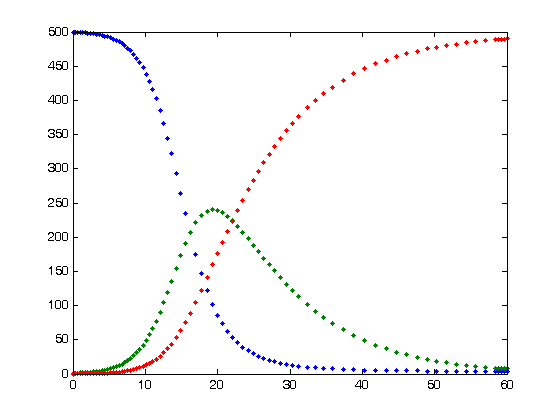
\includegraphics[width=0.5\textwidth]{figs/05/model-sir-data}\\
	\vspace{-0.5cm}
	\texttt{\tiny http://en.wikipedia.org/wiki/File:Sirsys-p9.png}
\end{figure}


\end{frame}

\begin{frame}{SIR is not the only model...}
%\begin{columns}
	% \begin{column}{0.45\textwidth}
		\begin{definition}[SIRS Model]
			The SIR model plus temporary immunity, so recovered nodes may
			become susceptible again.	
		\end{definition}
		\begin{figure}
			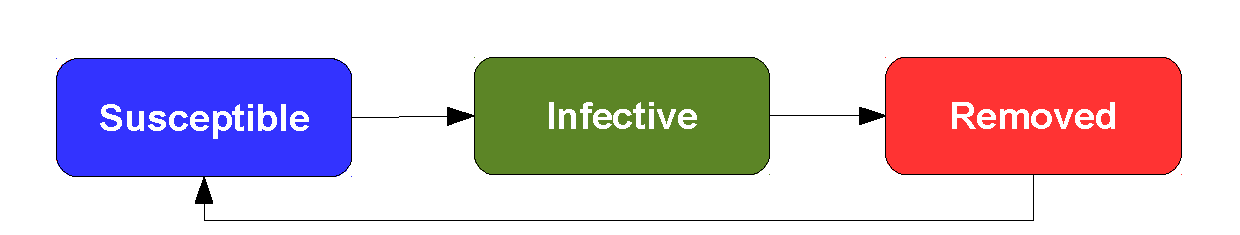
\includegraphics[width=0.6\textwidth]{figs/05/model-sirs}
		\end{figure}
	% \end{column}
	% \begin{column}{0.45\textwidth}
		\begin{definition}[SEIRS Model]
			The SEIRS model takes into consideration the \alert{exposed} or 
			latent period of the disease
		\end{definition}
		\begin{figure}
			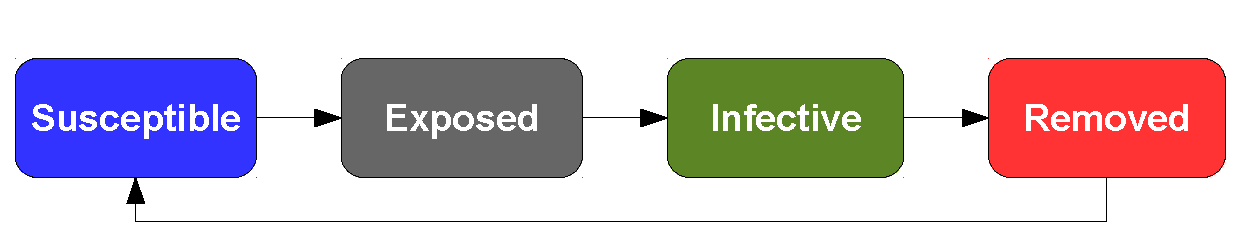
\includegraphics[width=0.6\textwidth]{figs/05/model-seirs}
		\end{figure}
% 	\end{column}
% \end{columns}	
\end{frame}

\begin{frame}{From Epidemiology to Distributed Systems}

\structure{The idea}

\BI
\item Disease spread quickly and robustly
\item Our goal is to spread an update as fast and as reliable as possible
\item Can we apply these ideas to distributed systems?
\EI

\bigskip
\begin{definition}[SIR Model for Database replication]
\BI
\item \alert{Susceptible}:	if $p$ has not yet received an update
\item \alert{Infective}:		if $p$ holds an update and is willing to share it
\item \alert{Removed}:	if $p$ has the update but is no longer willing to share it
\EI

\end{definition}

\bigskip
\structure{Note}: Rumor spreading, or gossiping, is based on the same principles


\end{frame}



\section{Algorithms}

\begin{frame}{Algorithm -- Summary}

\BIL
\item Best effort
\item \alert{Anti-entropy} (\alert{simple epidemics})
\BI
\item Push
\item Pull
\item Push-pull
\EI
\item \alert{Rumor mongering} (\alert{complex epidemics})
\BI
\item Push
\item Pull
\item Push-pull
\EI
\item Probabilistic broadcast
\EIL

\end{frame}

\subsection{Best-effort}

\begin{frame}{Best-effort}

\begin{block}{Best-effort (direct mail) algorithm}
\BI
\item Notify \textbf{all} other nodes of an update as soon as it
occurs. 
\item When receiving an update, check if it is “news” 
\EI
\end{block}

\begin{Procedure}
\caption{Direct mail protocol executed by process $p_i$:}
\UPON{$\Value_i \gets (v, \Now())$}{
 \ForEach{$p_j \in \Pi$}{
  \SEND $\langle \Update, \Value_i \rangle$ \TO $p_j$\;
 }
}
\BlankLine
\UPON{\RECEIVE $\langle \Update, (v,t) \rangle$}{
 \If{$\Value_i.\Time < t$}{
  $\Value_i \gets (v,t)$\;
 }
}
\end{Procedure}
\structure{Not randomized nor epidemic algorithm: just the simplest}

\end{frame}

\subsection{Anti-entropy}

\begin{frame}{Anti-entropy}
		
\begin{block}{Anti-entropy: Algorithm}
\BIL
\item Every node regularly chooses another node at random and exchanges 
database contents, resolving differences.
\item Nodes are either 
 \BI
 \item \alert{susceptible} -- they know the update
 \item \alert{infective} -- they know the update
 \EI
\EIL
\end{block}

\begin{Procedure}
\caption{Anti-entropy protocol executed by process $p_i$:}
\REPEAT{every $\Delta$ time units}{
 $\Process\ p_j \gets \Random(\Pi)$\Comment*[f]{Select a random neighbor}\;
 \{ exchange messages to resolve differences \}
}
\end{Procedure}

\end{frame}

\begin{frame}{Anti-entropy: graphical representation}
\begin{block}{Rounds}
During a \alert{round} of length $\Delta$
\BI
\item every node has the possibility of contacting one random node
\item can be contacted by several nodes
\EI
\end{block}

\begin{figure}
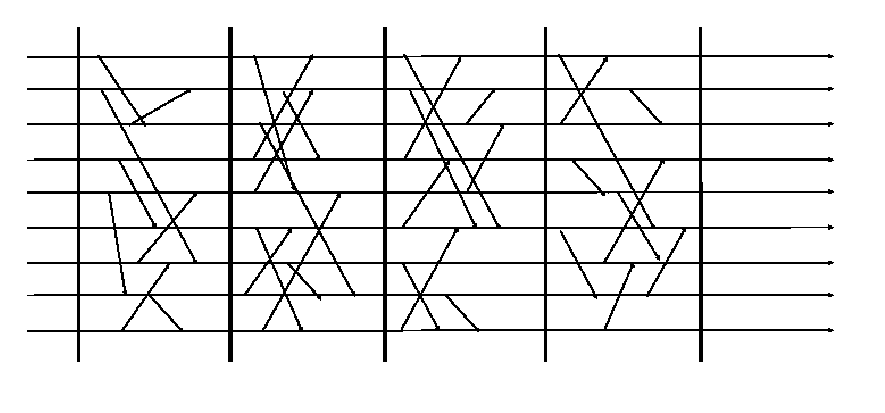
\includegraphics[width=0.8\textwidth]{figs/05/rounds}
\end{figure}

\end{frame}

\begin{frame}{Resolving differences -- Summary}
	
\begin{figure}
	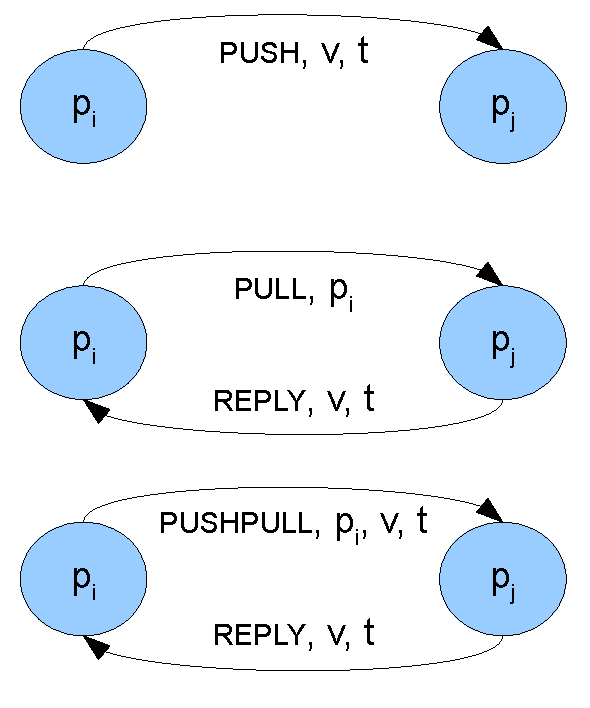
\includegraphics[width=0.4\textwidth]{figs/05/push-pull}
\end{figure}
	
\end{frame}

\begin{frame}{Resolving differences -- Push}

\begin{Procedure}
\caption{Anti-entropy, Push protocol executed by process $p_i$:}
\REPEAT{every $\Delta$ time units}{
 $\Process\ p_j \gets \Random(\Pi)$\Comment*[f]{Select a random neighbor}\;
 \SEND $\langle \Push, \Value_i \rangle$ \TO $p_j$\;
}
\BlankLine
\UPON{\RECEIVE $\langle \Push, (v, t) \rangle$}{
 \If{$\Value_i.\Time < t$}{
  $\Value_i \gets (v,t)$\;
 }
}

\end{Procedure}


\end{frame}

\begin{frame}{Resolving differences -- Pull}

\begin{Procedure}
\caption{Anti-entropy, Pull protocol executed by process $p_i$:}
\REPEAT{every $\Delta$ time units}{
 $\Process\ p_j \gets \Random(\Pi)$\Comment*[f]{Select a random neighbor}\;
 \SEND $\langle \Pull, p_i, \Value_i.\Time \rangle$ \TO $p_j$\;
}
\UPON{\RECEIVE $\langle \Pull, p_j, t \rangle$}{
 \If{$\Value_i.\Time > t$}{
 	\SEND $\langle \ReplyPull, \Value_i \rangle$ \TO $p_j$\;
  }
}
\BlankLine
\UPON{\RECEIVE $\langle \ReplyPull, (v, t) \rangle$}{
 \If{$\Value_i.\Time < t$}{
  $\Value_i \gets (v,t)$\;
 }
}
\end{Procedure}

\end{frame}


\begin{frame}{Resolving differences -- Push-Pull}

\begin{Procedure}
\caption{Anti-entropy, Push-Pull protocol executed by process $p_i$:}
\REPEAT{every $\Delta$ time units}{
 $\Process\ p_j \gets \Random(\Pi)$\Comment*[f]{Select a random neighbor}\;
 \SEND $\langle \PushPull, p_i, \Value_i \rangle$ \TO $p_j$\;
}
\BlankLine
\UPON{\RECEIVE $\langle \PushPull, p_j, (v, t) \rangle$}{
 \uIf{$\Value_i.\Time < t$}{
  $\Value_i \gets (v,t)$\;
 }
 \ElseIf{$\Value_i.\Time > t$}{
 	\SEND $\langle \ReplyPushPull, \Value_i \rangle$ \TO $p_j$\;
 }
}
\BlankLine
\UPON{\RECEIVE $\langle \ReplyPushPull, (v,t) \rangle$}{
 \If{$\Value_i.\Time < t$}{
  $\Value_i \gets (v,t)$\;
 }
}
\end{Procedure}

\end{frame}

\begin{frame}{Analytical results}

\begin{definition}[Compartmental model analysis]
We want to evaluate convergence of the protocol based on the size of the 
populations of susceptible and infected nodes (\alert{compartments})
\BI
\item $s_t$: the probability of a node being susceptible after $t$
 anti-entropy rounds
\item $i_t = 1 - s_t$: the probability of a node being infective after
$t$ anti-entropy rounds
\EI
\end{definition}

\begin{block}{Probability at round $k+1$}
\BIL
\item Initial condition: $s_0 = \onslide<2-5>{\frac{n-1}{n}}$
\item Pull: $E[s_{t+1}] = \onslide<3-5>{s_{t}^2}$
\item Push: $E[s_{t+1}] = \onslide<4-5>{s_{t}(1-\frac{1}{n})^{(1-s_{t})n}} \onslide<5>{\approx s_{t} e^{-(1-s_{t})}}$
\EIL
\end{block}

\note{
\begin{minipage}{\textwidth}
\BI
\item Probability at round 0: 1 node is infective, all the others $n-1$ are susceptible
\item In case of pull, a node will remain susceptible at round $t+1$ if it was susceptible 
 at round $t$ (prob.: $s_t$) and it contacts a susceptible node (prob.: $s_t$).
\item In case of push, a node will remain susceptible at round $t+1$ if it was susceptible 
 at round $t$ (prob.: $s_t$) and it is \textbf{not} selected randomly (prob: $1-\frac{1}{n}$) by
all nodes that are not susceptible, which are $(1-s_t)n$.
\EI
\end{minipage}
}

\end{frame}

\begin{frame}{Analytical results}

\begin{definition}[Termination time]
Let $S_n$ be the first cycle where $s_t=0$ in a population of $n$ individuals 
\BI
\item \alert{Push}: Pittel (1987) shows that in probability, $S_n = \log n + \ln n + O(1)$
\item \alert{Push-pull}: Karp et al. (2000) shows that in probability, $S_n = \log \log n$
\EI
\end{definition}

\bigskip
{\footnotesize
\structure{Relevant bibliography}:
\BI
\item B. Pittel. \alert{On spreading a rumor}. SIAM Journal of Applied Mathematics, 47(1):213–223, 1987.
\item R. Karp, C. Schindelhauer, S. Shenker, B. Vocking. \alert{Randomized
rumor spreading}. In Proc. the $41^{\textrm{st}}$ Symp. on
Foundations of Computer Science, 2000.
\EI
}

\note{
\BI
\item The proof is rather long and technical, but the intuitive explanation is rather 
simple.  
\item In the initial cycles, most nodes are susceptible. 
\item In this phase, the number of infected nodes will 
double in each cycle to a good approximation. 
\item However, in the last cycles, where $s_t$ is small, we can see that $E[s_{t+1}] \approx s_te^{-1}$.
\item This suggests that there is a first phase, lasting for approximately $\log_2 n$ cycles
\item There is a last phase lasting for $\ln N$ cycles. 
\item The middle phase, between these two phases, can be shown to be very fast, lasting a constant number of cycles.
\EI

}


\end{frame}


\begin{frame}{Analytical results}

\structure{In summary:}

All methods converge to $0$, but pull and push-pull are much more rapid

\begin{figure}
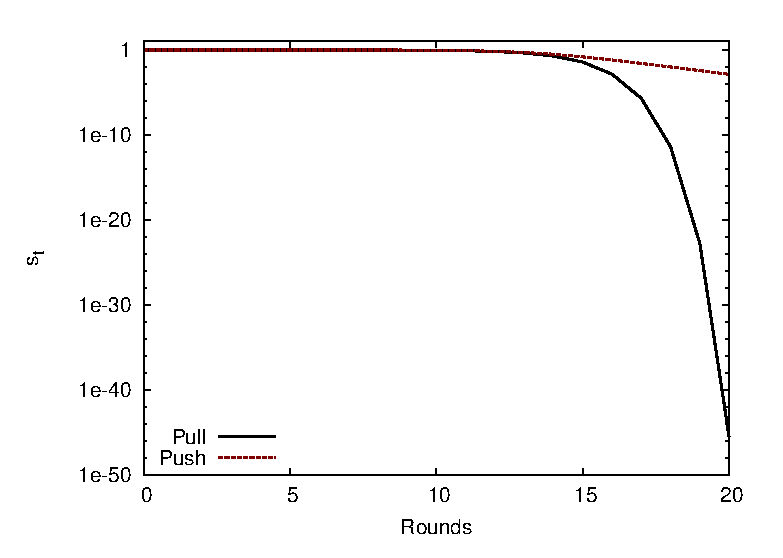
\includegraphics[width=0.6\textwidth]{figs/05/gnuplot}
\caption{$n=10\,000$}
\end{figure}

\end{frame}

\begin{frame}{Comments}
	
\begin{block}{Benefits}
\BI
\item Simple epidemic eventually “infects” all the population
\item It is extremely robust
\EI
\end{block}

\bigskip
\begin{block}{Drawbacks}
\BI
\item Propagates updates much slower than direct mail (best effort)
\item Requires examining contents of database even when most data agrees, so it cannot practically be used too often
\item Normally used as support to best effort/rumor mongering, i.e. left running in the background
\EI
\end{block}

\end{frame}

\begin{frame}{Working with multiple values}
	
\structure{Examples of techniques to compare databases:}	
	
\BIL
\item Maintain checksum, compare databases if checksums unequal
\item Maintain recent update lists for time $T$, exchange lists first
\item Maintain inverted index of database by timestamp; exchange information in reverse timestamp order, incrementally re-compute checksums
\EIL

\smallskip
\structure{Notes}:

\BIL
\item Those ideas apply to databases
\item Strongly application-dependent
\item We will see how anti-entropy may be used beyond information dissemination
\EIL

\end{frame}

\subsection{Rumor-mongering}

\begin{frame}{Rumor mongering in brief}
	
\BIL
\item Nodes initially “susceptive”
\item When a node receives a new update it becomes a “hot rumor” and the node “infective”
\item A node that has a rumor periodically chooses randomly another node to spread the rumor
\item Eventually, a node will “lose interest” in spreading the rumor and becomes “removed”
\BI
 \item Spread too many times
 \item Everybody knows the rumor
\EI
\item A sender can hold (and transmit) a list of infective updates rather than just one
\EIL

\end{frame}

\begin{frame}{Rumor mongering: loss of interest }

\BIL
\item \textbf{When}: Counter vs coin (random)
\BI
\item \alert{Coin} (\alert{random}): lose interest with probability $1/k$
\item \alert{Counter}: lose interest after $k$ contacts
\EI
\item \textbf{Why}: Feedback vs blind
\BI
\item \alert{Feedback}: lose interest only if the recipient knows the rumor.
\item \alert{Blind}: lose interest regardless of the recipient.
\EI
\EIL
\end{frame}

\begin{frame}{Analytical results}

\begin{block}{Question}
How fast does the system converge to a state where all nodes are not infective? (inactive state)
\end{block}

\structure{Compartmental analysis again -- Feedback, coin}

Let $s$, $i$ and $r$ denote the fraction of susceptible, infective, and removed nodes, respectively. Then:
\begin{eqnarray*}
s + i + r &=& 1\\
ds/dt &=& – si\\
di/dt &=& +si –\frac{1}{k}(1 – s)i
\end{eqnarray*}

\structure{Solving the differential equations}: 
\BI
\item $s = e^{-(k+1)(1-s)}$
\item Increasing $k$ increases the probability that the nodes get the
rumor
\EI

\note{
\BI
\item $si$ corresponds to the proportion of nodes that are \emph{susceptible} and
are contacted by \emph{infective} nodes at any given round
\item $ds/dt = -si$ and $di/dt = +si$ mean that those nodes will be not susceptible any more and
will become infective
\item $-(1/k)(1-s)i$ means that with probability $\frac{1}{k}$, an infective
node ($i$) will become removed if it contacts a non-susceptible node $(1-s)$.
\EI

}

\end{frame}

\begin{frame}{Quality measures}
	
\begin{definition}[Residue]
\BI
\item The nodes that remain susceptible when the epidemic ends: value of $s$ when $i = 0$.
\item Residue must be as small as possible
\EI
\end{definition}

\begin{definition}[Traffic]
\BI
\item The average number of database updates sent between nodes
\item $m$ = total update traffic / \# of nodes
\EI
\end{definition}

\begin{definition}[Convergence]
\BI
\item $t_\mathit{avg}$ : average time it takes for all nodes to get an update
\item $t_\mathit{last}$ : time it takes for the last node to get the update
\EI
\end{definition}
\end{frame}

\begin{frame}{Simulation results}
	
\begin{figure}
	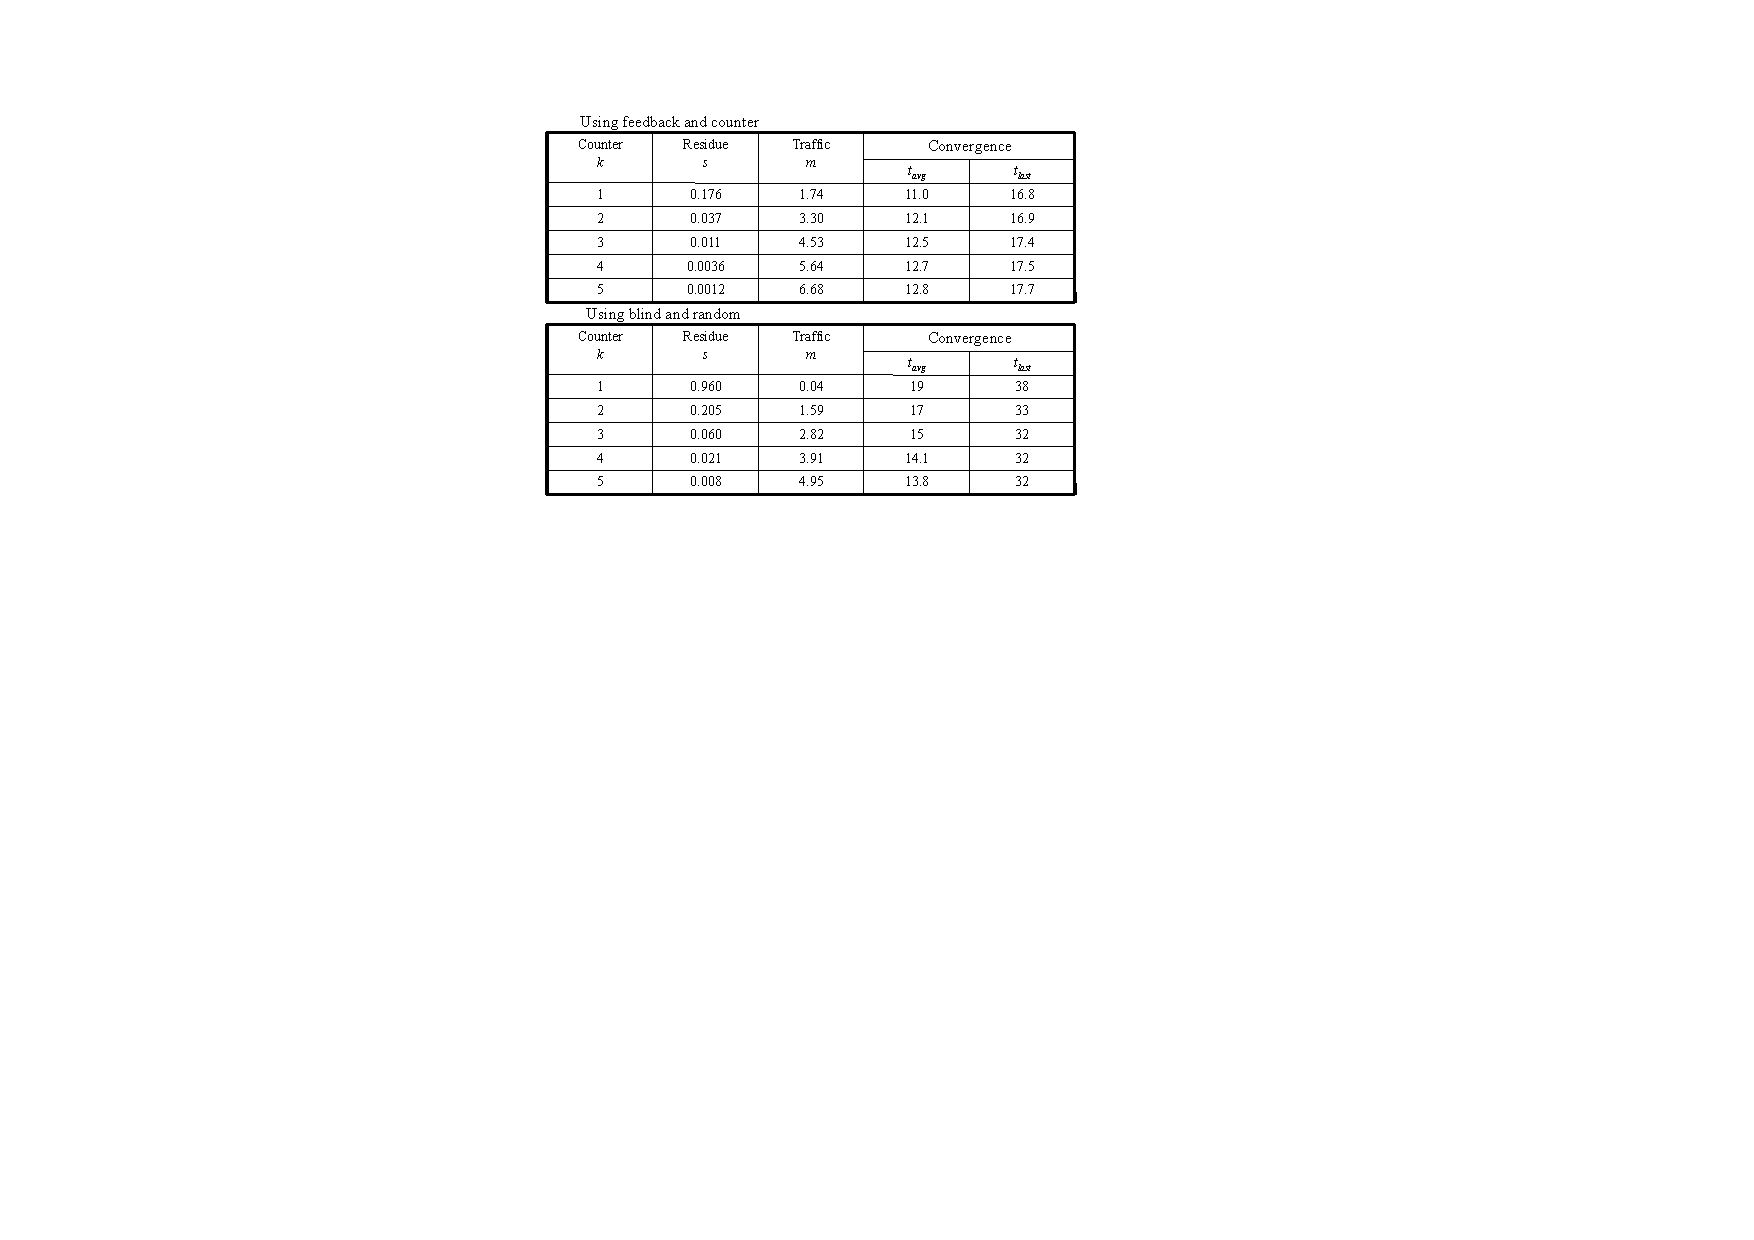
\includegraphics[width=0.8\textwidth]{figs/05/simulation}	
\end{figure}

\end{frame}

\begin{frame}{Push vs pull}
	
\BIL
\item Push (what we have assumed so far)
\BI
\item If the database becomes quiescent, push stops trying to introduce updates
\EI
\item Pull
\BI
\item If many independent updates, pull is more likely to find a source with a non-empty rumor list
\item But if the database is quiescent, several update requests are wasted
\EI
\EIL

\end{frame}

\begin{frame}{Rumor Mongering + Anti-Entropy}

\BIL
\item Quick \& Dirty Push Rumor Mongering 
\BI
\item spreads updates fast with low traffic.
\item however, there is still a nonzero probability of nodes remaining susceptible after the epidemic
\EI
\item Not-so-fast Push-Pull Anti-Entropy
\BI
\item can be run (infrequently) in the background to ensure all nodes eventually get the update with probability $1$
\EI
\EIL

\end{frame}

\subsection{Deletion and death certificates}

\begin{frame}{Dealing with deletions}

\begin{block}{Deletion}
\BI
\item We cannot delete an entry just by removing it from a node - the absence
of the entry is not propagated
\item If the entry has been updated recently, there may still be an update
traversing the network!
\EI
\end{block}

\begin{definition}[Death certificate]
Replace the deleted item with a \alert{death certificate} that has a timestamp
and spreads like an ordinary update.
\end{definition}

\end{frame}

\begin{frame}{Dealing with deletions}

\begin{block}{Problem}
We must, at some point, delete DCs or they may consume significant space
\end{block}

\BIL
\item \textbf{Strategy 1}: retain each DC until all nodes have received it
\BI
\item requires a protocol to determine which nodes have it and to handle node failures
\EI

\item \textbf{Strategy 2}: hold DCs for some time (e.g. 30d) and discard them
\BI
\item pragmatic approach
\item we still have the “resurrection” problem
\item increasing the time requires more space
\EI
\EIL

\end{frame}

\begin{frame}{Dormant certificates}

\structure{Observation}:

\BI
\item we can delete very old DCs but retain only a few “dormant” copies in some nodes
\item if an obsolete update reaches a dormant DC, it is “awakened” and re-propagated
\EI

\bigskip
\structure{Analogy with epidemiology}:
 
\BI
\item the awakened DC is like an antibody triggered by an immune reaction
\EI

\end{frame}

\subsection{Probabilistic broadcast}

\begin{frame}{Epidemics vs probabilistic broadcast}
	
\structure{Anti-entropy}:

DB is a collection of message received

\bigskip
\structure{Rumor mongering}

Updates $\equiv$ Message broadcast

\end{frame}

%%%%%%%%%%%%%%%%%%%%%%%%%%%%%%%%%%%%%%%%%%%%%%%%%%%%%%%%%%%%%%%%%%%%%%%%

\section{What's next}

\begin{frame}{What's next?}

\begin{block}{Problems}
\BI
\item \alert{Membership}:\\How do processes get to know each other, and how many do 
they need to know?
\item \alert{Network awareness}:\\ How to make the connections between processes reflect the actual 
network topology such that the performance is acceptable? 
\item \alert{Buffer management}:\\
Which updates to drop when the storage buffer of a process is full? 
\EI
\end{block}


\begin{block}{Does not end here...}
Epidemic/gossip approach has been successfully applied to other problems. 
We will provide a brief overview of them.
\end{block}

\end{frame}

\nocite{demers87}
\nocite{gossip11}
\ReadingMaterial

\end{document}
